\documentclass{beamer}
\usetheme{Boadilla} 
\setbeamercovered{invisible}
\setbeamertemplate{navigation symbols}{} 
%\useoutertheme{infolines} 

\usepackage[utf8]{inputenc}
\usepackage{graphicx}

\setbeamertemplate{frametitle continuation}{} 
\usepackage{subfigure}
\usepackage{caption}
\usepackage{bm}
\usepackage{epsfig}

\usepackage{amsmath}
\usepackage{xcolor,colortbl}

\usepackage{multicol}
\usepackage{wasysym}

\usepackage{hyperref}
\usepackage{float}

\usepackage{array}
\newcolumntype{L}[1]{>{\raggedright\let\newline\\\arraybackslash\hspace{0pt}}m{#1}}
\newcolumntype{C}[1]{>{\centering\let\newline\\\arraybackslash\hspace{0pt}}m{#1}}
\newcolumntype{R}[1]{>{\raggedleft\let\newline\\\arraybackslash\hspace{0pt}}m{#1}}

% deal with spaces in absolute paths

\usepackage[space]{grffile}
\graphicspath{{C:/Users/Yered/Dropbox/Harvard/Winter 2014/CdeC/Slides/Introduction/figures/}}

\usepackage[scaled]{helvet}
\usepackage[round]{natbib}
\usepackage{courier}

\begin{document}
\title[Introducción a R \& RStudio]{Explorando el Transcriptoma con Datos de Expresi\'{o}n Gen\'{e}tica\\
\vspace{0.5cm}
Introducción a R \& RStudio}
\author{Yered Pita-Ju\'{a}rez}
\institute[CdeC M\'{e}rida]{}
\date{3/1/2015}

\begin{frame}
\titlepage
\end{frame}

\begin{frame}{¿Qué es R?}
\begin{itemize}
\item R es un lenguaje de programación para el análisis estadístico
\item La interacción con R es a través de una línea de comandos
\item R es software libre
\end{itemize}
\begin{figure}[H]
\centering

\includegraphics[scale=0.35]{R-logo.png}
\end{figure}
\end{frame}

\begin{frame}{Ventajas de R}
\begin{itemize}
\item R es gratis
\item Existe una gran comunidad trabajando para mejorarlo constantemente
\item Disponible para Windows, OS, Linux/Unix
\item R es actualizado frequentemente
\item R es sumamente potente y versátil, gracias a la gran disponibilidad de \textit{packages}
\item R es un estándar en el análisis de datos genómicos
\item \textcolor{red}{Utiliza  línea de comandos en lugar de un interfaz gráfico}
\end{itemize}
\begin{center}
{\Huge \smiley}
\end{center}
\end{frame}

\begin{frame}{Desventajas de R}
\begin{itemize}
\item La documentación es amplia, pero a veces puede resultar confusa
\item R no da muchas pistas acerca de qué puede estar fallando
\item Algunos \texttt{packages} han sido ampliamente probados, otros no tanto
\item \textcolor{red}{Utiliza  línea de comandos en lugar de un interfaz gráfico}
\end{itemize}
\begin{center}
{\Huge \frownie}
\end{center}
\end{frame}

\begin{frame}{Instalando R}
\begin{itemize}
\item Descarga \& instala R\\
\url{http://cran.r-project.org/}
\end{itemize}
\begin{figure}[H]
\centering
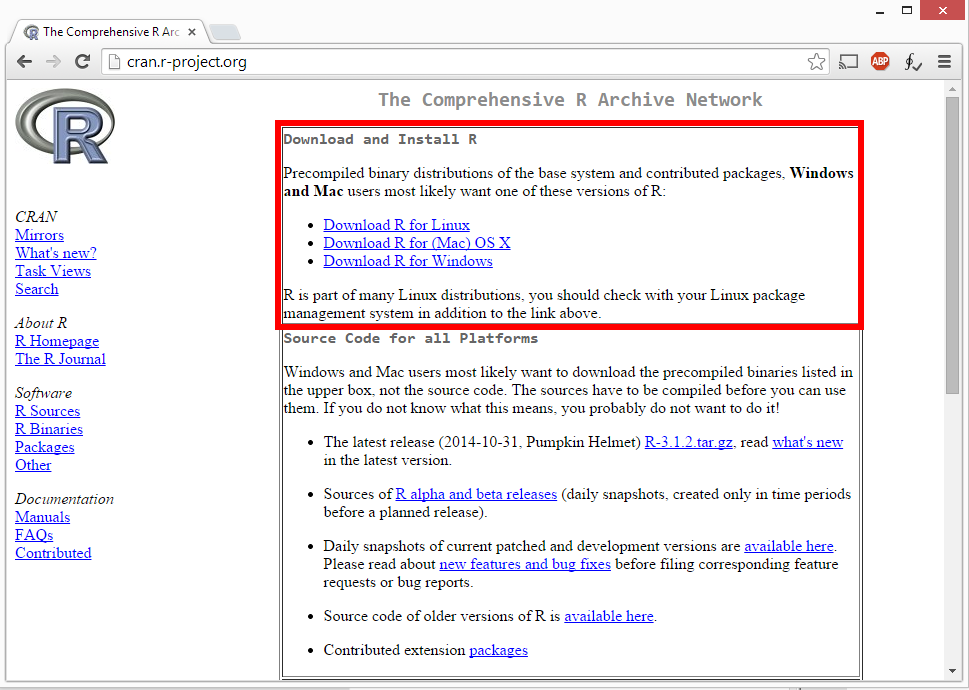
\includegraphics[scale=0.35]{cran_website00.PNG}
\end{figure}
\end{frame}

\begin{frame}{Instalando R}
\begin{itemize}
\item Descarga \& instala R\\
\url{http://cran.r-project.org/}
\end{itemize}
\begin{figure}[H]
\centering
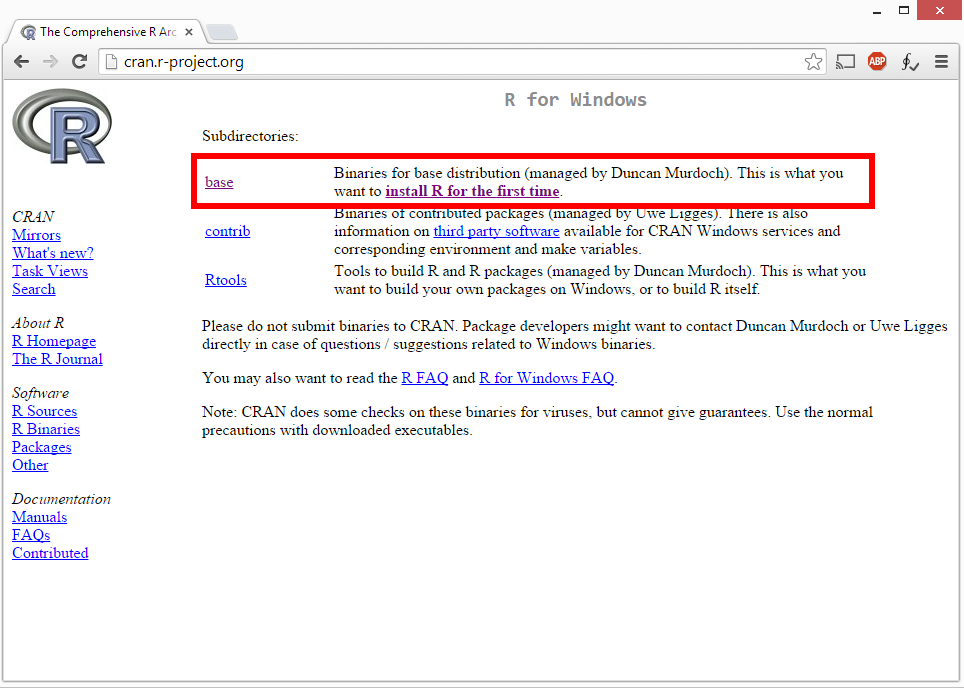
\includegraphics[scale=0.35]{cran_website01.PNG}
\end{figure}
\end{frame}

\begin{frame}{Instalando R}
\begin{itemize}
\item Descarga \& instala R\\
\url{http://cran.r-project.org/}
\end{itemize}
\begin{figure}[H]
\centering
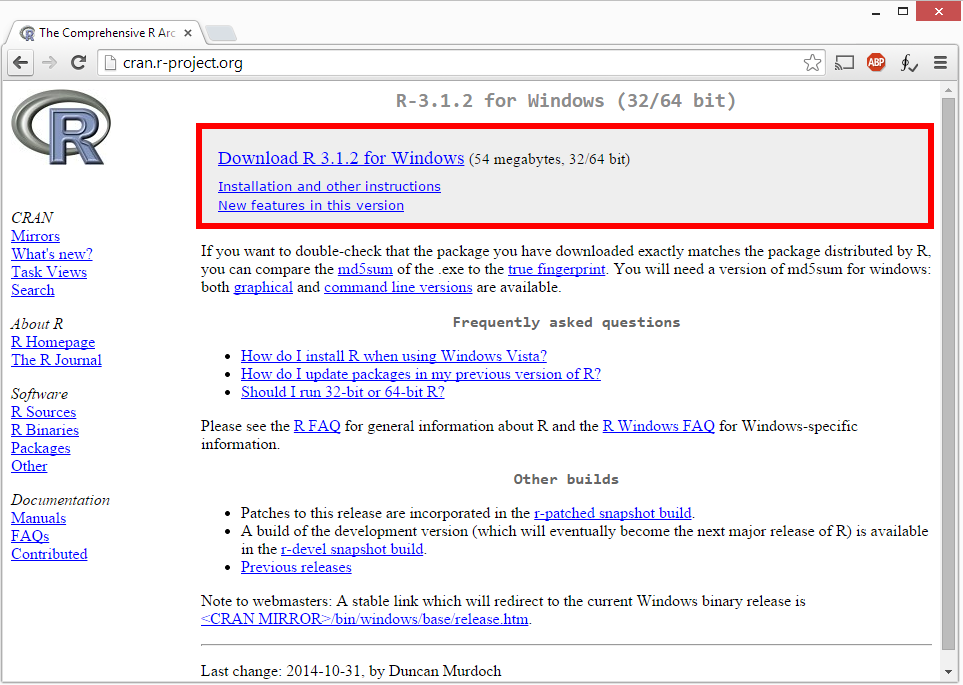
\includegraphics[scale=0.35]{cran_website02.PNG}
\end{figure}
\end{frame}

\begin{frame}{Instalando R}

\begin{figure}
\begin{tabular}{cc}
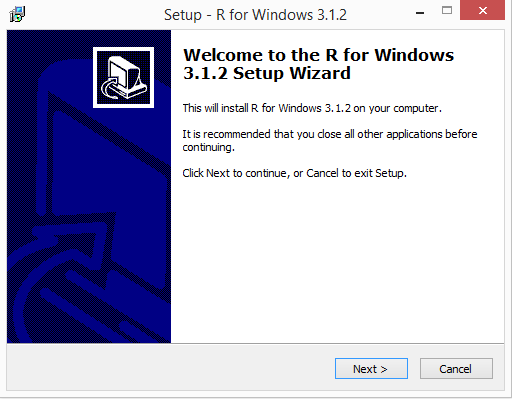
\includegraphics[width=0.35\linewidth]{install_R00.png} &   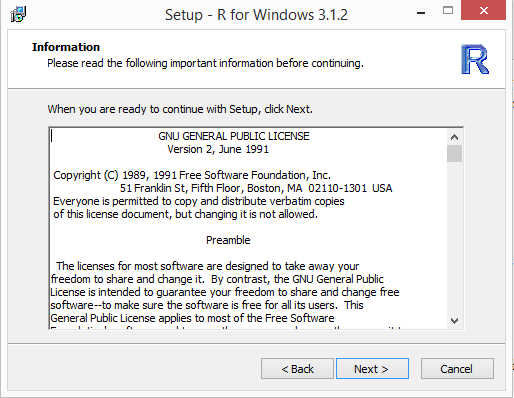
\includegraphics[width=0.35\linewidth]{install_R01.png} \\
1 & 2\\
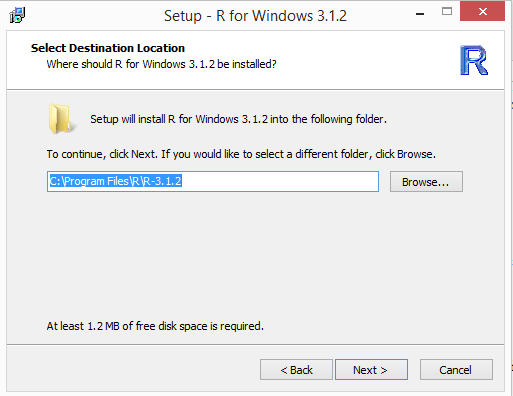
\includegraphics[width=0.35\linewidth]{install_R02.png} &  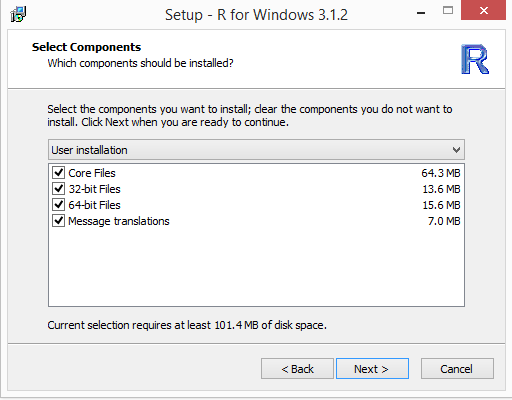
\includegraphics[width=0.35\linewidth]{install_R03.png} \\
3 & 4\\
\end{tabular}
\end{figure}
\end{frame}

\begin{frame}{RStudio}
\begin{itemize}
\item La interface de R puede ser díficil de usar
\begin{figure}[H]
\centering
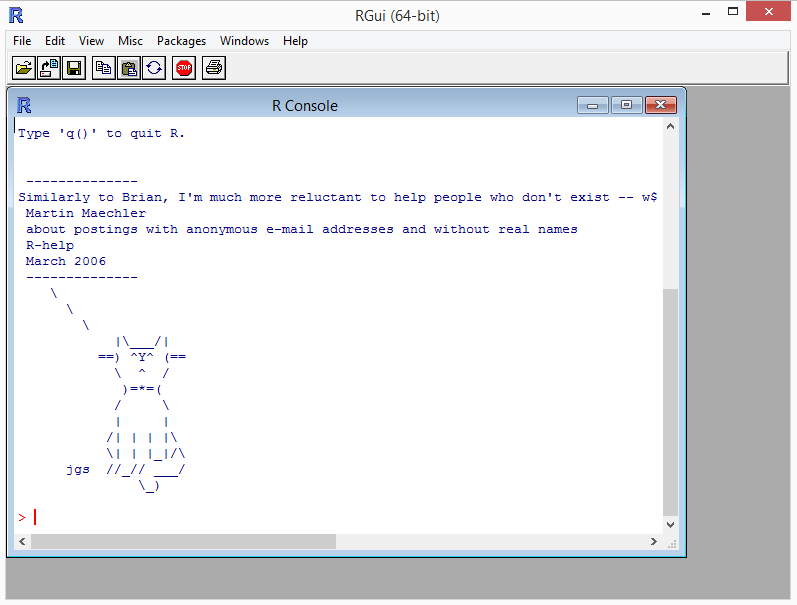
\includegraphics[scale=0.25]{R_gui.png}
\end{figure}
\item Vamos a usar RStudio como la interface para R\\
\url{http://www.rstudio.com/}
\begin{figure}[H]
\centering

\includegraphics[scale=0.5]{RStudio-logo.png}
\end{figure}
\end{itemize}
\end{frame}

\begin{frame}{Instalando RStudio}
\begin{itemize}
\item Descarga \& instala RStudio\\
\url{http://www.rstudio.com/}
\begin{figure}[H]
\centering
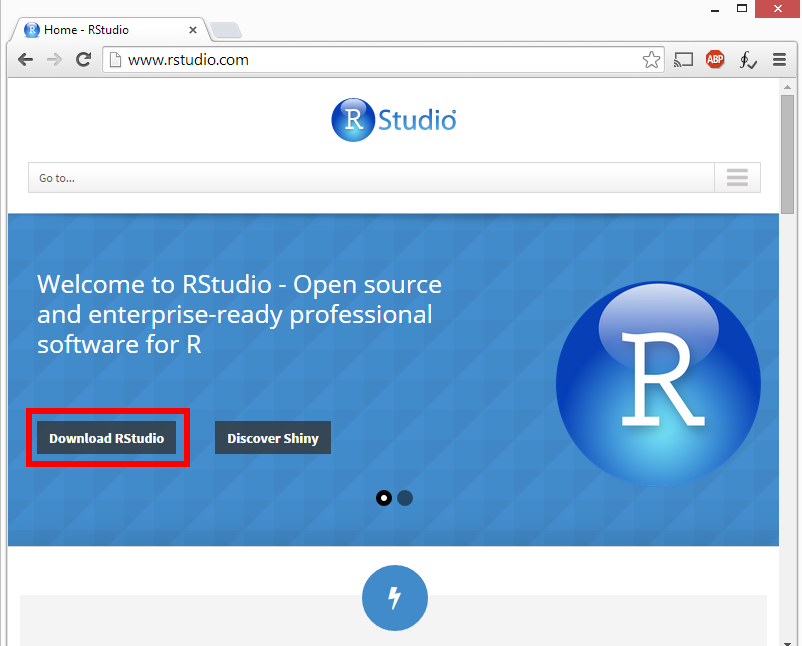
\includegraphics[scale=0.35]{RStudio_website00.PNG}
\end{figure}
\end{itemize}
\end{frame}

\begin{frame}{Instalando RStudio}
\begin{itemize}
\item Descarga \& instala RStudio\\
\url{http://www.rstudio.com/}
\begin{figure}[H]
\centering
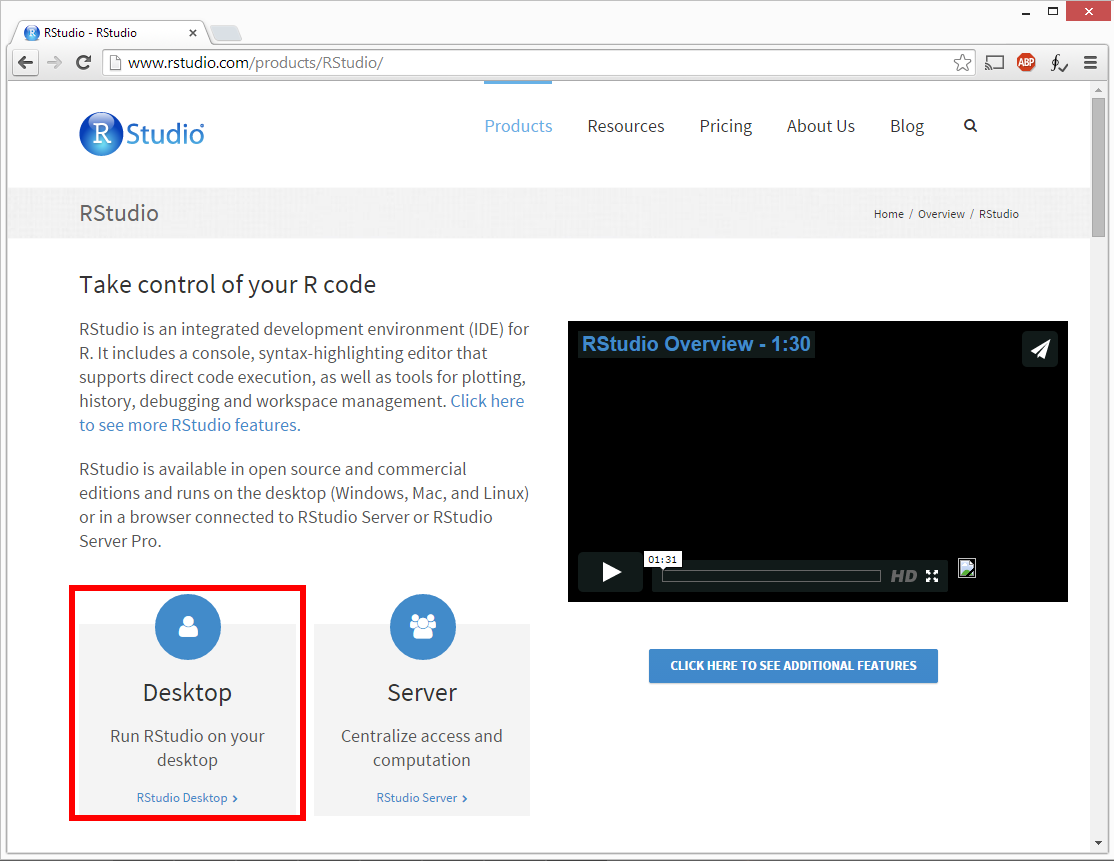
\includegraphics[scale=0.25]{RStudio_website01.PNG}
\end{figure}
\end{itemize}
\end{frame}

\begin{frame}{Instalando RStudio}
\begin{itemize}
\item Descarga \& instala RStudio\\
\url{http://www.rstudio.com/}
\begin{figure}[H]
\centering
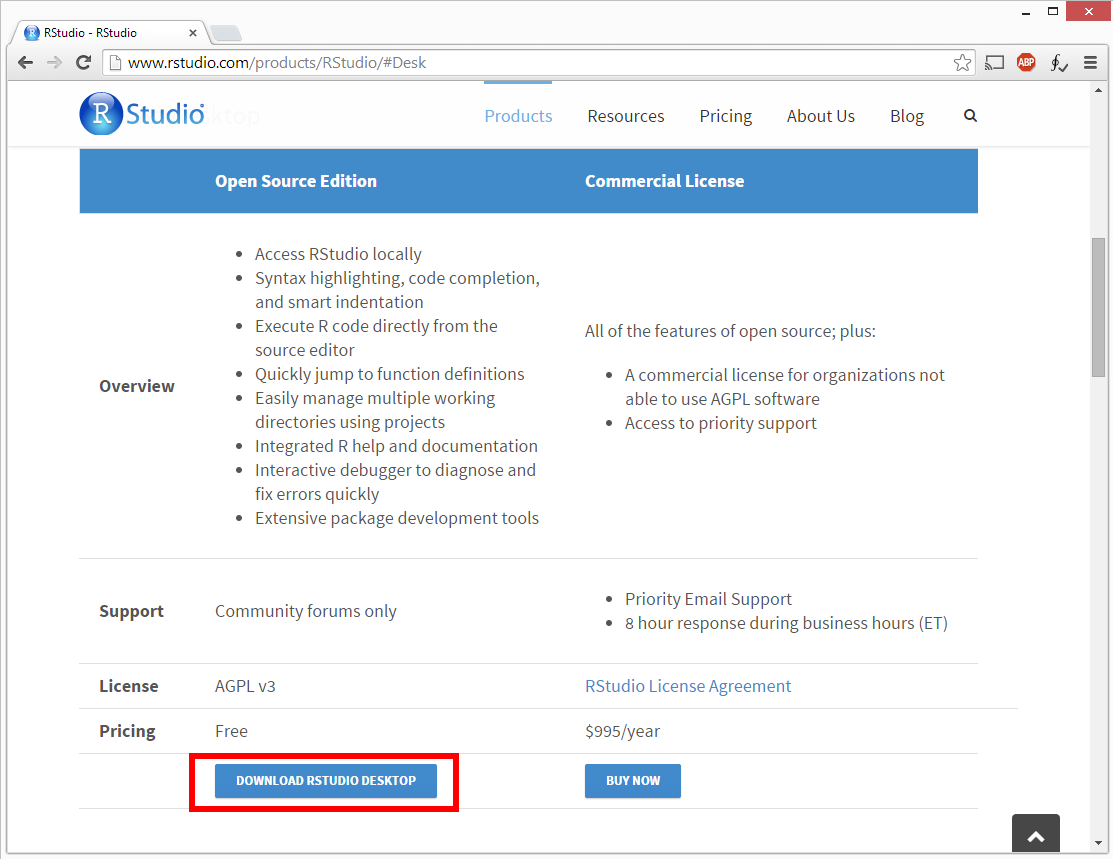
\includegraphics[scale=0.25]{RStudio_website02.PNG}
\end{figure}
\end{itemize}
\end{frame}

\begin{frame}{Instalando RStudio}
\begin{itemize}
\item Descarga \& instala RStudio\\
\url{http://www.rstudio.com/}
\begin{figure}[H]
\centering
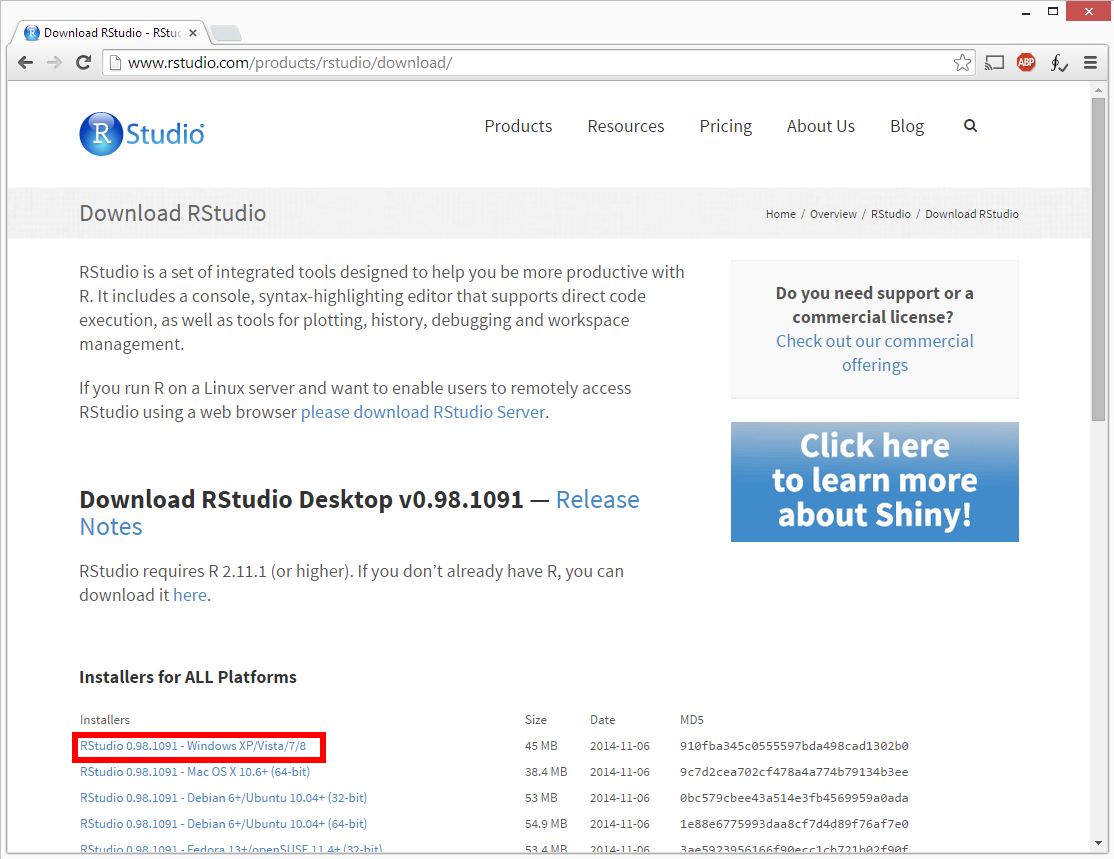
\includegraphics[scale=0.25]{RStudio_website03.PNG}
\end{figure}
\end{itemize}
\end{frame}

\begin{frame}{Instalando RStudio}

\begin{figure}
\begin{tabular}{cc}
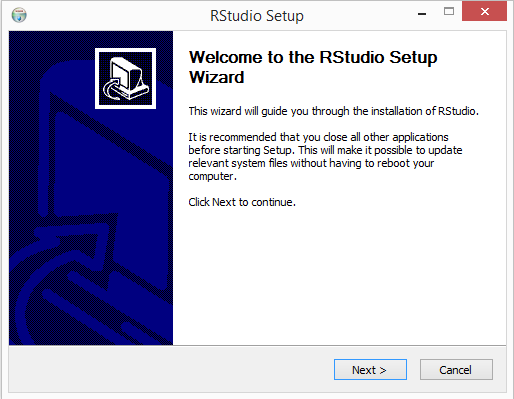
\includegraphics[width=0.35\linewidth]{install_RStudio00.png} &   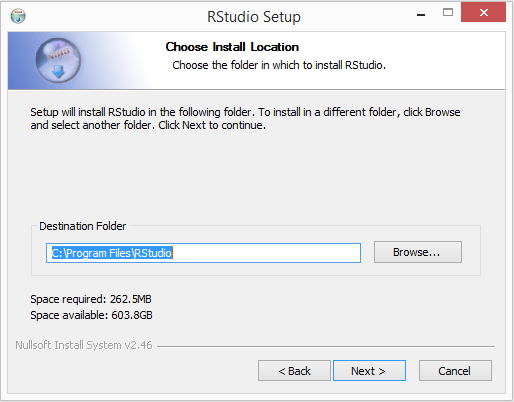
\includegraphics[width=0.35\linewidth]{install_RStudio01.png} \\
1 & 2\\
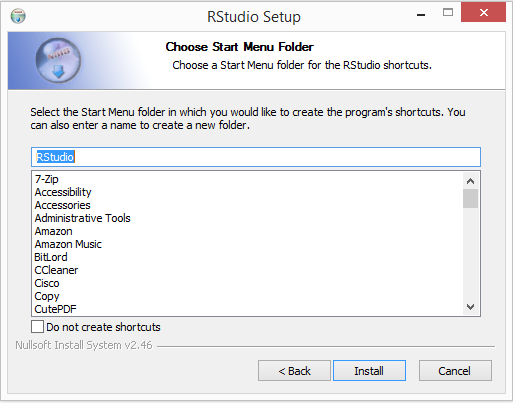
\includegraphics[width=0.35\linewidth]{install_RStudio02.png} &   \\
3 & \\
\end{tabular}
\end{figure}
\end{frame}

\begin{frame}{RStudio}
\begin{itemize}
\item RStudio tiene 4 paneles principales
\begin{enumerate}
\item \textbf{editor panel (script panel)}
\item \textbf{console panel (command panel)}
\item \textbf{workspace/history panel}
\item \textbf{files/plots/packages/help panel}
\end{enumerate}
\begin{figure}[H]
\centering
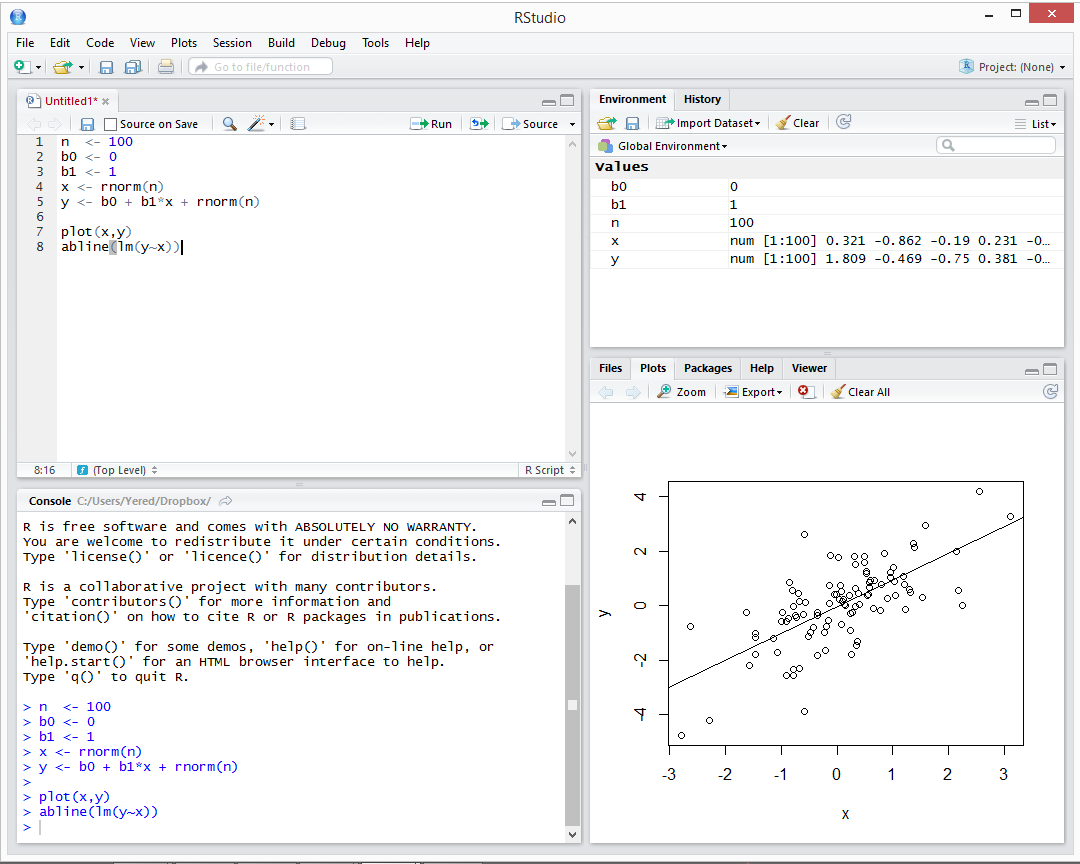
\includegraphics[scale=0.65]{rstudio_screen.png}
\end{figure}
\end{itemize}
\end{frame}

\begin{frame}{RStudio}
\begin{itemize}
\item \textbf{editor panel (script panel):} para editar y guardar conjuntos de comandos (scripts)
\end{itemize}
\begin{figure}[H]
\centering
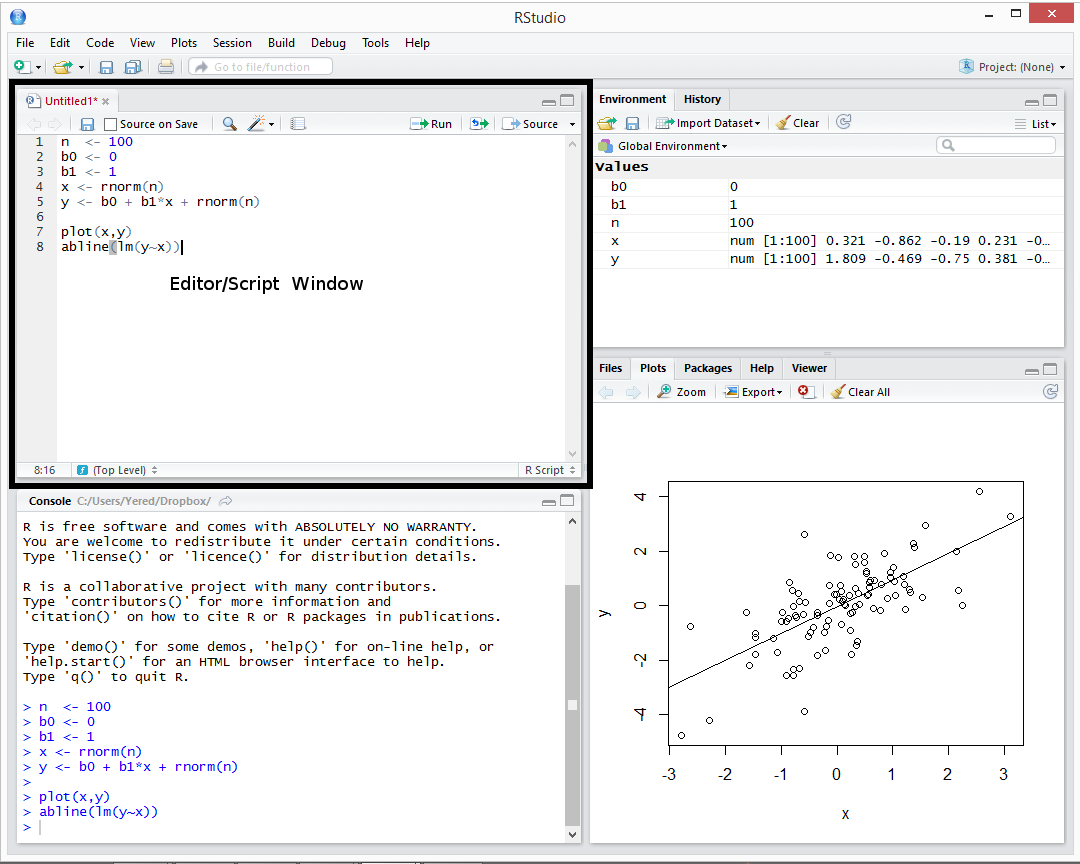
\includegraphics[scale=0.85]{rstudio_screen01.png}
\end{figure}
\end{frame}

\begin{frame}{RStudio}
\begin{itemize}
\item \textbf{console panel:} el panel más importante de R, aquí se ejecutan los comandos 
\end{itemize}
\begin{figure}[H]
\centering
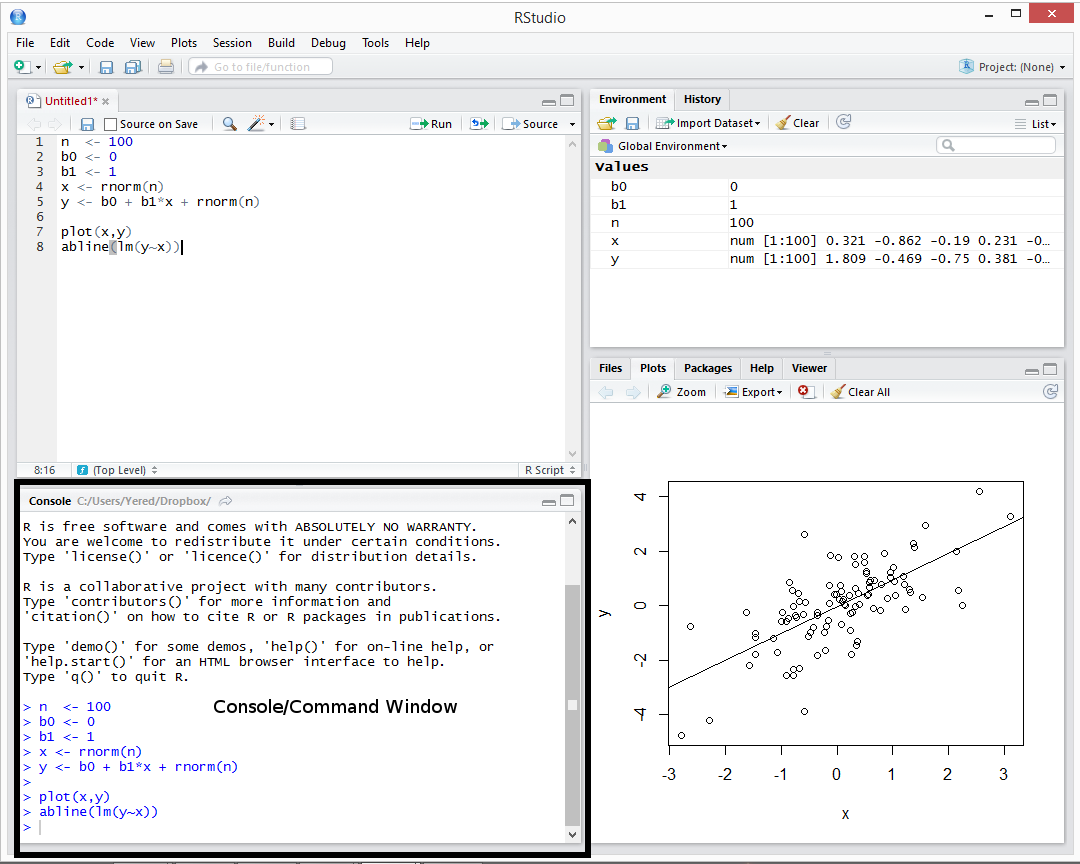
\includegraphics[scale=0.85]{rstudio_screen02.png}
\end{figure}
\end{frame}

\begin{frame}{RStudio}
\begin{itemize}
\item \textbf{workspace/history panel:} el panel \textbf{workspace} tiene que datos y objectos R contiene en la memoria, el panel \textbf{history} tiene los comandos que han sido ejecutados anteriormente
\end{itemize}
\begin{figure}[H]
\centering
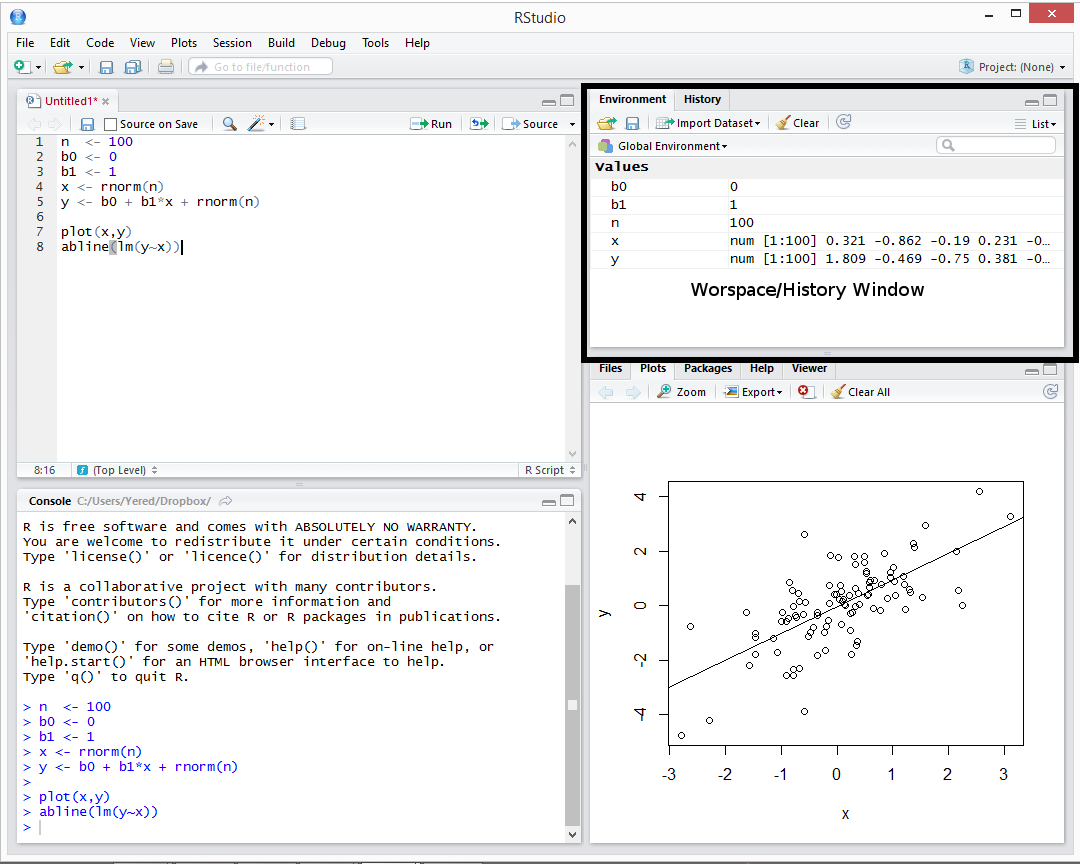
\includegraphics[scale=0.85]{rstudio_screen03.png}
\end{figure}
\end{frame}

\begin{frame}{RStudio}
\begin{itemize}
\item \textbf{files/plots/packages/help panel:} aquí puedes abrir archivos, ver gráficos, instalar y cargar \texttt{packages} o usar la función de ayuda
\end{itemize}
\begin{figure}[H]
\centering
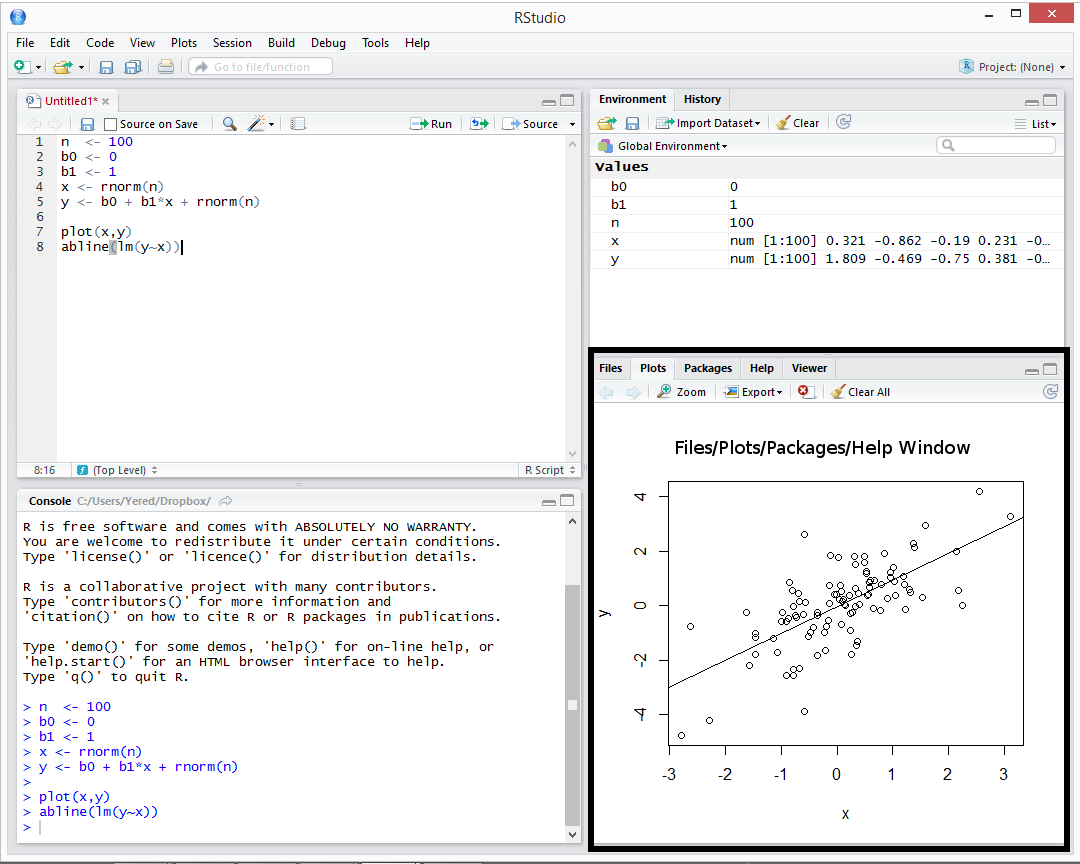
\includegraphics[scale=0.85]{rstudio_screen04.png}
\end{figure}
\end{frame}
\end{document} 

